\documentclass[11pt]{article}
\usepackage{amsmath}
%\usepackage{extsizes}
\usepackage{amsmath,amssymb}
%\usepackage{omegavn,ocmrvn}
%\usepackage[utf8x]{inputenc}
\usepackage[utf8]{vietnam}

\usepackage{listings}
\lstset{language=Python}          % Set your language (you can change the language for each code-block optionally)


\usepackage{longtable}
\usepackage{answers}
\usepackage{graphicx}
\usepackage{array}
\usepackage{pifont}
\usepackage{picinpar}
\usepackage{enumerate}
\usepackage[top=3.0cm, bottom=3.5cm, left=3.5cm, right=2.5cm] {geometry}

\usepackage{extarrows}
\usepackage{hyperref}


\newtheorem{bt}{Câu}
\newcommand{\RR}{\mathbb R}
\Newassociation{sol}{Solution}{ans}
\newtheorem{ex}{Câu}
\renewcommand{\solutionstyle}[1]{\textbf{ #1}.}


\begin{document}
% \noindent

\begin{tabular*}
	{\linewidth}{c>{\centering\hspace{0pt}} p{.7\textwidth}}
	Trường ĐHKHTN, ĐHQGHN & {\bf Học Kỳ 2 (2021-2022)}
	\tabularnewline
	K64 TTƯD - Thầy Hà Phi & {\bf Bài Tập Giải Tích Số \\ \today}
	% Exercises on pages 239, 240 Cheney/Kincaid are really nice
	\tabularnewline
	\rule{1in}{1pt}  \small  & \rule{2in}{1pt} %(Due date:)
	\tabularnewline
	%  \tabularnewline
	%  &(Đề thi có 1 trang)
\end{tabular*}




\begin{center}
	{\bf Bài Thi Giữa Kỳ - Tính Toán Khoa Học}
\end{center}

\begin{bt}
a) Thế nào là hệ LTI? hệ LTV? Hai hệ này khác nhau thế nào? \\
b) Công thức hàm truyền của hệ LTI là gì?
\end{bt}

\begin{bt} 
Tính chất ổn định của điểm cân bằng là gì? Lấy ví dụ minh họa cho tính ổn định và không ổn định.
\end{bt}

\begin{bt}
a) Phương trình Lyapunov có dạng nào. Điều kiện tồn tại duy nhất nghiệm của nó là gì. Phát biểu thuật toán giải phương trình Lyapunov. \\
b) Phương trình Sylvester có dạng nào. Điều kiện tồn tại duy nhất nghiệm của nó là gì. Phát biểu thuật toán giải phương trình Sylvester.
\end{bt}

\begin{bt}
Có mấy cách biểu diễn một hệ thống điều khiển? Mô hình không gian trạng thái, mô hình hàm truyền, mô hình zpk là gì?
\end{bt}

\begin{bt} Các hệ thống sau có điều khiển được hay không? Vì sao? Tìm hàm truyền của các hệ thống đó. \\
a) \textbf{Dạng chính tắc điều khiển được (controllability canonical form)}
%
\begin{align}
	\dot{x} &= \m{0 & 1 & &  & \\ &  \ddots & \ddots &  & \\ & & \ddots & \ddots &   \\&  &  & 0 & 1 \\ -\a_1 & -\a_2 & \dots & \dots & -\a_{r} } x + \m{0 \\ \vdots \\ \vdots \\ 0 \\ 1} u, \\
y &= \m{\b_1 &  \dots & \dots & \b_r} x + D u, 
\end{align}
%
trong đó $\a_i$, $\b_i$, $D$ là các hệ số (thực hoặc phức). \\
b) \textbf{Dạng chính tắc quan sát được (observability canonical form)}
%
\begin{align}
	\dot{x} &= \m{-\a_1 & 1 & &  & \\ \vdots &   & \ddots &  & \\ \vdots & & & \ddots &   \\ -\a_{r-1} &  &  &  & 1 \\ -\a_{r} & 0 & \dots & \dots & 0} x + \m{\b_1 \\  \vdots \\ \vdots \\ \b_{r-1} \\ \b_r} u, \\
y &= \m{1 &  0 & \dots & \dots & 0} x + D u, 
\end{align}
%
trong đó $\a_i$, $\b_i$, $D$ là các hệ số (thực hoặc phức). \\
c) \textbf{Bài toán nhận dạng (relization problem): Cho trước hàm truyền, đi tìm dạng không gian trạng thái.} \\
Hãy tổng quát hóa các dạng chính tắc ở trên, sao cho hàm truyền của hệ có dạng 
%
\begin{equation}
	G(s) = D + \dfrac{\b_r s^{r-1} + \dots + \b_2 s + \b_1}{s^r + \a_r s^{r-1} + \dots + \a_{2} s + \a_1} \ ,
\end{equation}
%
trong đó $r \leq n$. Ở đây $G(s)$ được gọi là 1 hàm chính thường, \textbf{proper function}.
\end{bt}

\begin{bt} \textbf{Nghiên cứu về tính điều khiển được của 2 hệ thống được mắc nối tiếp/song song với nhau theo các sơ đồ trong Hình \ref{fig:electricalconnection}.} \\

\begin{figure}[!h]
	\centering
	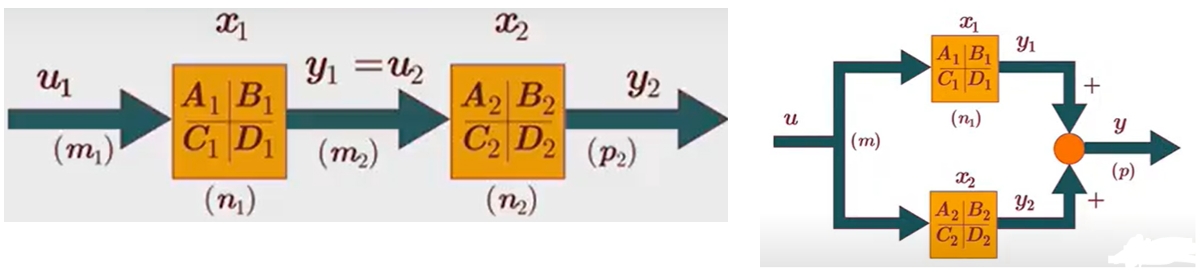
\includegraphics[scale = 0.6]{Figures/Electrical_connection}
	\caption{Mạch nối tiếp (trái) \& Mạch song song (phải)}
	\label{fig:electricalconnection}
\end{figure}

\noindent Giả sử rằng các hệ con đều là điều khiển được. \\
1) Hãy xây dựng phương trình của hệ thống mắc nối tiếp, chú ý rằng ở đây đầu vào của hệ tổng chỉ có $u_1$, và đầu ra của hệ tổng là $y_2$. Chứng minh rằng nếu hệ thống tổng là điều khiển được thì nó không thể có vector riêng trái dạng $w = \m{w_1 & 0} \in \C^{n_1+n_2}$ mà thỏa mãn điều kiện $w^H B= 0$ . \\
2) Hãy xây dựng phương trình của hệ thống song song. Chứng minh hệ thống song song sẽ đánh mất tính điều khiển được khi và chỉ khi $A_1$ và $A_2$ có giá trị riêng chung $\lambda$, và các vector riêng trái $w_1$, $w_2$ tương ứng thỏa mãn
\begin{align*}
	& w^H_1 B_1 + w^H_2 B_2 = 0, \\
	& w^H_1 A_1 = \lambda w^H_1,   \   w^H_2 A_2 = \lambda w^H_2.
\end{align*}
\end{bt}


\begin{bt} \textbf{Bài tập lập trình} \\
\end{bt}   

	
\end{document}



